\documentclass[12pt]{article}
\usepackage[utf8]{inputenc}
\usepackage[english]{babel}
\usepackage{graphicx}
\usepackage{float}
\usepackage{amsmath}
\usepackage[table]{xcolor}
\usepackage{xcolor}
\usepackage{enumitem}
\usepackage{titlesec}
\usepackage{amssymb}
\usepackage{cancel}

\title{Homework 4}
\author{Leonard David Vivas Dallos \\ Mariana Valencia Cubillos \\ Samuel Mira Álvarez}
\date{\today}

\begin{document}

\maketitle
\textbf{\textit{Assignment:}} Write solutions for exercises 2(c) and 13(c)

\tableofcontents

\renewcommand{\thesubsection}{\thesection.\alph{subsection}}

\setcounter{section}{1}

\section{Exercise 2}

\setcounter{subsection}{2}

Let $G = (V, \Sigma, R, S)$ be the context-free grammar, where $V = \{S\}$, $\Sigma = \{0, 1\}$, $S$ is the start variable, and $R$ consists of the rules
\begin{equation*}
    S \rightarrow SS | 00S1 | 1S00 | 0S1S0 | \varepsilon
\end{equation*}

\begin{enumerate}
    \item[a)] Determine $L(G)$
    \item[b)] Give a $PDA$ that accepts $L(G)$
    \item[c)] Give a grammar for the case of $3$ (the qeustion should be clear after doing the first part).
\end{enumerate}

\subsection{Solution}

\begin{align*}
S &\rightarrow A \mid B \mid C \\
A &\rightarrow 1A \mid \varepsilon \quad \text{(cualquier número de '1')} \\
B &\rightarrow 11B \mid \varepsilon \quad \text{(cualquier número par de '1')} \\
C &\rightarrow 111C \mid \varepsilon \quad \text{(cualquier número impar de '1')}
\end{align*}

c) Give a grammar for the case of 3.
\vspace{5pt}

\textbf{Proof Idea:} We now want a grammar that generates the language
\(L_{\text{triple}}\), which is just alike \(L_{\text{double}}\), but in
this case, we want the number of 0's to triplicate the number of 1's in
the string. Formally, we define
\(L_{\text{triple}} = \left\{ w \in \left\{ 0,1 \right\}^{*}\  \right|\ \#(0,w) = 3\  \cdot \#(1,w)\}\).
The idea is that, seeming that the language we wish to generate is like
the one we just did, we can tweak slightly the grammar we were already
given to make one that fits our needs.

It seems that the grammar for \(L_{\text{double}}\) used the
possibilities of where can the 1 be placed in a chain of two 0s. In that
case, it could either be in the beginning, in the end, or in between.
That's easy enough, but now we have an uneven number of 0s, moreover, we
have one more 0 to worry about. However, we can follow the same idea.
Let's play the same game and think where we can place the 1 in that
string of 3 0s. Again, we can place it in the end or the beginning of
the 0s, but now, when we want to place it in between, we must take in
account in which part of the ``between'' we want to put it in. That
leaves us with two possibilities: Leaving two 0s to the left of the 1
and one 0 to the right of it; or, contrarily, leaving one 0 to the left
of the 1 and two 0s to the right. However, it is not enough to know
this, we must also know where we must collocate the variable in the new
rules, such that they, indeed, generate all combinations of strings in
\(L_{\text{triple}}.\) For that, look carefully at the rules next
presented, and note that every rule can be interpreted as ``How many 0s
do each rule produce to the left and right sides of the 1?''. Therefore,
if you had any string that fulfills the condition for being in
\(L_{\text{triple}}\), you can generate it with the grammar by carefully
seeing the amount of 0s that separate two 1s, and using rules in a way
such that you leave between the 1s the number of 0s desired.

Let \(G' = (V^{'},\Sigma,R^{'},S')\) be a context-free grammar, where
\(V^{'} = \{ S^{'}\}\), \(\Sigma = \{ 0,1\}\), \(S'\) is the start
variable, and \(R'\) comprises the rules:

\[S^{'} \rightarrow S^{'}S^{'}\left| 000S^{'}1 \right|1S^{'}000\left| 0S^{'}1S^{'}00 \right|00S^{'}1S^{'}0|\varepsilon\]

\textbf{Proof: Let's prove that}
\(\mathbf{L}\left( \mathbf{G}^{\mathbf{'}} \right)\mathbf{=}\mathbf{L}_{\mathbf{\text{triple}}}\)\textbf{.}

\[\mathbf{L}\left( \mathbf{G}^{\mathbf{'}} \right)\mathbf{\subseteq}\mathbf{L}_{\mathbf{\text{triple}}}\]

Intuitively, this is straightforward. Note that every rule in \(S'\)
introduces three 0s and one 1. Let's prove it mathematically by
induction over the length of derivation \(l\) of the string \(w\).

\textbf{Base case:} We say that there is a string \(w\) in \(L(G^{'})\) with
length of derivation \(l = 1\) and we prove that
\(w \in L_{\text{triple}}\) too. A string in \(L(G^{'})\) with length of
derivation \(l = 1\) is \(\varepsilon\), since
\(S^{'} \Rightarrow \varepsilon\) and \(\varepsilon\) is a string
(albeit an empty one). However, \(\varepsilon \in L_{\text{triple}}\)
since \(\#(0,\varepsilon) = 0 = 3 \cdot 0 = 3 \cdot \#(1,\varepsilon)\).
Therefore, it holds true.

\textbf{Induction Hypothesis:} We suppose that for any string \(x\) of length of
derivation \(l^{'} < l\), it holds true that \(x \in L(G^{'})\) and
\(x \in L_{\text{triple}}\).

\textbf{Inductive Step:} Now, we assume that there is a string \(w \in L(G^{'})\)
and with length of derivation \(l\). We want to show that
\(w \in L_{\text{double}}\).

Now, we consider the following ways of yielding \(w\):

\(S^{'} \Rightarrow S^{'}S^{'} \Rightarrow^{*}w\): Then,
\(w = xy\ \)with
\(S' \Rightarrow^{m}x\ \)and\(\text{\ S}' \Rightarrow^{n}y;\ m,\ n < l\text{.\ }\)By
Induction Hypothesis, \(x,y \in L_{\text{triple}}\), and therefore,
\(w = xy \in L_{\text{triple}}\),
since\(\ \#(0,\ w)\  = \ \#(0,\ x) + \#(0,\ y)\  = \ 3 \cdot \#(1,\ x) + 3 \cdot \#(1,\ y) = \ 3 \cdot \left( \#(1,\ x) + \#(1,\ y) \right) = 3 \cdot \#(1,\ w)\).

\(S^{'} \Rightarrow 000S^{'}1 \Rightarrow^{*}w\): Then, \(w = 000x1\),
with \(S^{'} \Rightarrow^{l - 1}x\). By Induction Hypothesis,
\(x \in L_{\text{triple}}\), and therefore,
\(w = 000x1 \in L_{\text{triple}}\), since
\(\#(0,w) = 3 + \#(0,x) = 3 + 3 \cdot \#(1,x) = 3\left( 1 + \#(1,x) \right) = 3 \cdot \#(1,w)\).

\(S^{'} \Rightarrow 1S'000 \Rightarrow^{*}w\): Then, \(w = 1x000\), with
\(S^{'} \Rightarrow^{l - 1}x\). By Induction Hypothesis,
\(x \in L_{\text{triple}}\), and therefore,
\(w = 000x1 \in L_{\text{triple}}\). The analysis is analogous to the
case before.

\(S^{'} \Rightarrow 0S^{'}1S'00 \Rightarrow^{*}w\): Then,
\(w = 0x1y00\), with
\(S' \Rightarrow^{m}x\ \)and\(\text{\ S}' \Rightarrow^{n}y;\ m,\ n < l\).
By Induction Hypothesis, \(x,y \in L_{\text{triple}}\), and therefore,
\(w = 0x1y00 \in L_{\text{triple}}\). The analysis is a combination of
the first and second cases.

\(S^{'} \Rightarrow 00S^{'}1S'0 \Rightarrow^{*}w\): Then,
\(w = 00x1y0\), with
\(S' \Rightarrow^{m}x\ \)and\(\text{\ S}' \Rightarrow^{n}y;\ m,\ n < l.\)
By Induction Hypothesis, \(x,y \in L_{\text{triple}}\), and therefore,
\(w = 00x1y0 \in L_{\text{triple}}\). The analysis is a combination of
the first and second cases.

In either case, we've shown that
\(w \in L\left( G^{'} \right) \Rightarrow w \in L_{\text{triple}}.\)

\[\mathbf{L}_{\mathbf{\text{triple}}}\mathbf{\subseteq}\mathbf{L(}\mathbf{G}^{\mathbf{'}}\mathbf{)}\]

This one is \textbf{not} straightforward. This is so hard please help.

We want now to see that if there is a string \(w \in L_{\text{triple}}\)
with length \(|w|\), then \(w \in L\left( G^{'} \right)\text{.\ }\)

This time, we \textbf{claim} that \(w\) can be written in either way:

\begin{center}
    \(xy, 000x1, 1x000, 0x1y00, 00x1y0,\)     
\end{center}

with each \(x,y \in L_{\text{triple}}\) and \(|x|,|y| < |w|\). Therefore, there
must be possible, using the derivation rules of \(G'\), to yield \(w\).

Proof of \textbf{claim:} By induction over the length of
\(w;\ |w| = n\). For this proof, we will also use a function \(g\) with
domain \(\left\{ m \in \mathbb{N} \right|m \leq n\}\):

\[g(i) = \#(0,w\lbrack 1:i\rbrack) - 3\#(1,w\lbrack 1:i\rbrack)\]

Remember that \(w\lbrack k,j\rbrack\) is the substring of \(w\) starting
in \(w_{k}\) and going until \(w_{j}\). Again, this is a function that
measures the excess of 0s over thrice the amount of 1s in the prefix of
\(w\) of length \(i\). Also, note that \(g(0) = 0\) (since no symbols
have been read yet), and \(g(n) = 0\) (since all symbols have been read,
and since \(w \in L_{\text{triple}}\), it should have thrice the amount
of 0s than the amount of 1s). Very importantly, notice that, when
``reading'' a symbol (i.e., when we go from \(g(i)\) to \(g(i + 1)\)),
the function can only go up by 1, or go down by 3 (in words of the
demonstration of 2.a, \(g(i + 1) - g(i)\) is either 1 (if 
\(w\lbrack i\rbrack = 0\)) or \(-\)3 (if \(w\lbrack i\rbrack = 1\))).

\textbf{Base case:} \(|w| = 0\). Trivial, since
\(\varepsilon \in L_{\text{triple}}\) (remember that
\(\#(0,\varepsilon) = 0 = 3 \cdot 0 = 3 \cdot \#(1,\varepsilon))\) and
\(S' \Rightarrow \varepsilon\), meaning,
\(\varepsilon \in L\left( G^{'} \right).\)

\textbf{Induction Hypothesis:} For any string \(x\), with \(|x| < n\), it holds
true that \(x \in L_{\text{triple}} \Rightarrow x \in L(G^{'})\).

\textbf{Inductive Step:} Now suppose \(|w| \geq 4.\) Similarly, to 2.a), we will
consider the cases for the combinations of symbols in the furthermost
sides of the string \(w\). One of the following must hold true:

\textit{Case 1:} Assume \(w\) starts and ends in a 0. Then \(g(1) = 1\) and
\(g(n - 1) = - 1\). Intuitively, the function \(g\) must go from
positive to negative at some point. We consider the following subcases:

\begin{itemize}
\item
  \textit{Subcase 1.1:} Function \(g\) goes from positive to negative by taking a
  value of \(0\). Then, there must be a number \(m < n\) where
  \(g(m) = 0\), and therefore, \(w\lbrack 1,m\rbrack\) and
  \(w\lbrack m + 1,n\rbrack\) both have the number 0s three times the
  number of 1s. Then, \(w\) can be split into two strings, that is,
  \(w = xy\), with \(|x|,|y| < |w|\) and, by induction hypothesis,
  \(x,y \in L\left( G^{'} \right).\) Then, \(w\) is also in
  \(L\left( G^{'} \right)\) (\(w\) is yielded by the rule
  \(S^{'} \Rightarrow S'S'\)).
\item
  \textit{Subcase 1.2:} Function \(g\) goes from positive to negative not by
  taking a value of 0. That is, for some \(k < n\), \(g(k)\) is either 1
  or 2, and then, \(g(k + 1)\) is either -2 or -1, (by ``reading'' a 1).
  If function \(g\) goes from 1 to -2, then \(w\lbrack 2,k\rbrack = x\)
  and \(w\lbrack k + 1,n - 2\rbrack = y\) must be substrings with the
  number of 0s three times the number of 1s (since \(g(1) = g(k)\) and
  \(g(k + 1) = g(n - 2)\), because if not, then \(g(n - 2) = 2\)
  (\(w\lbrack n - 2\rbrack = 1\)) meaning that the function must've gone
  positive at one point, and since it can only do it by adding 1, then
  there would be another index \(j < n\) in which \(g(j) = 0\),
  contradicting our assumption), and as \(|x|,|y| < |w|\), by Induction
  Hypothesis, \(x,y \in L(G^{'})\) and, then,
  \(w \in L\left( G^{'} \right)\) (\(w\) is yielded by the rule
  \(S^{'} \Rightarrow 0S^{'}1S'00\)). If \(g\) foes from 2 to -1
  instead, then, \(w\lbrack 3,k\rbrack = x\) and
  \(w\lbrack k + 1,n - 1\rbrack = y\) must be sub-strings with the number
  of 0s three times the number of 1s (similarly to before,
  \(g(k + 1) = g(n - 1)\) and \(g(3) = g(k)\), because if it weren't
  true, there would be an index at which the function \(g\) would've
  gone positive again, doing so by taking a value of 0, contradicting
  the assumption that \(g\) does not go from positive to negative by
  taking a 0), and since \(|x|,|y| < |w|\), by Induction Hypothesis,
  \(x,y \in L(G^{'})\) and, then, \(w \in L\left( G^{'} \right)\) (\(w\)
  is yielded by the rule \(S^{'} \Rightarrow 00S^{'}1S'0\)).
\end{itemize}

\textit{Case 2:} Assume \(w\) starts and ends in a 1. Then \(g(1) = - 3\) and
\(g(n - 1) = 3\). Observe again that \(g\) must go from negative to
positive at some point. Since function \(g\) can only go up by 1 unit
each time, that means that at some index \(k < n\), \(g(k) = 0\). Then,
similarly to Sub-case 1.1, there are sub-strings
\(w\lbrack 1,k\rbrack = x\) and \(w\lbrack k + 1,n\rbrack = y\) both
having the number 0s three times the number of 1s and having a lower
length. By Induction Hypothesis, \(x,y \in L(G^{'})\), and then
\(w = xy \in L(G^{'})\) (\(w\) is yielded by the rule
\(S^{'} \Rightarrow S'S'\)).

\textit{Case 3:} Assume \(w\) starts with a 1 and ends in a 0. Then,
\(g(1) = - 3\) and \(g(n - 1) = - 1\). If the function \(g\) were to go
positive at some point, it would be doing so at some index \(k < n\),
meaning that we would have the same case as Case 2. However, we must
also verify the cases where \(g\) doesn't go positive. Note that, then,
\(g(n - 2) = - 2\), \(g(n - 3) = - 3\) (since, if that weren't true,
then either \(g(n - 2) = 1\) or \(g(n - 3) = 0\), and that leaves us
with the case before, where \(g\) touches \(0\) and can then be divided
in two strings containing triple the number of 0s than 1s). Therefore,
there must be \(w\lbrack 2,n - 3\rbrack = x\) must be a substring of
\(w\) containing thrice the number of 0s than the number of 1s. By
Induction Hypothesis, \(x \in L(G^{'})\), and then, \(w \in L(G^{'})\)
(\(w\) is yielded by the rule \(S^{'} \Rightarrow 1S'000\)).

\textit{Case 4:} Assume \(w\) starts with a 0 and ends in a 1. Then, \(g(1) = 1\)
and \(g(n - 1) = 3\). Similarly to Case 3, if \(g\) were to have a
negative value at some point, that means that it would have to go
negative and positive again. Since the transition from negative to
positive can only be done by steps of +1, then for some index \(k < n\),
\(g(k) = 0\), and we would again have a similar case of that of Case 2,
and we could divide \(w\), and it would then be yielded by
\(S' \Rightarrow S'S'\). Now, let's consider the cases where \(g\) does
not take a negative value. Then, again, note that \(g(2) = 2\) and
\(g(3) = 3\) (because, if that weren't true, then either \(g(2) = - 1\)
or \(g(3) = 0\), which, once again, allows for \(w\) to be split in two
strings that are in \(L_{\text{triple}}\)). Then,
\(w\lbrack 4,n - 1\rbrack = x\) is a string that must contain three
times the number of 0s than the number of 1s. Then, \(x \in L(G^{'})\)
by Induction Hypothesis; and from that follows that \(w \in L(G^{'})\)
(\(w\) is yielded by the rule \(S^{'} \Rightarrow 000S^{'}1)\).

In any case, \(w\) may be written in the form

\begin{center}
    \(xy,\ 1x000,\ 0001x,\ 0x1y00,\ 00x1y0,\)    
\end{center}

with \(|x|,|y| < |w|\) and
\(x,y \in L_{\text{triple}}\), meaning, that \(w\) may be written in the
form of any of the rules of \(G'\), or in other words, that for any
\(w \in L_{\text{triple}}\), \(S' \Rightarrow^{*}w\).

That concludes the proof that
\(L\left( G^{'} \right) = L_{\text{triple}}\).
\(\ \ \ \ \ \ \blacksquare\)

\setcounter{section}{12}

\section{Exercise 13}

Let $\Sigma = \{0, 1\}$ and $\Sigma_{\#} = \{ 0, 1, \# \}$.
\begin{enumerate}
    \item[a)] Consider the languages:
        \begin{flalign*}
            A &= \{ x\#x^R | x\in \Sigma^* \} \\
            B &= \{ x \# x | x \in \Sigma^* \}
        \end{flalign*}
        Determine for each of $A$, $B$ and their complements whether it is a CFL.
    \item[b)] Let
        \begin{equation*}
            C = \{x \# x^R \# x | x \in \{ 0, 1 \} ^* \}
        \end{equation*}
        Show that the complement of $C$ is a CFL
    \item[c)] For a positive integer, let $[i]_2$ denote its corresponding binary representation with a leading $1$. Let
        \begin{flalign*}
            D &= \{ [i]_2 \# [i+1]_2^R | i \geq 1 \} \\
            E &= \{ [i]_2 \# [i+1]_2 | i \geq 1\}
        \end{flalign*}
        Determine for each of $D$, $E$ and their complements whether it is a CFL.
\end{enumerate}

\setcounter{subsection}{2}

\subsection{Solution}

\textit{\textbf{\begin{enumerate}
    \item $D$ is a CFL.
\end{enumerate}}}

\begin{figure}[h]
    \centering
    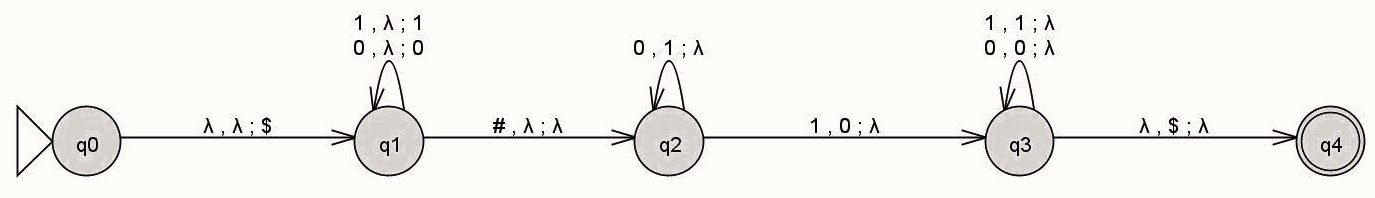
\includegraphics[width=0.9\linewidth]{Tarea 4 PDA D.jpg}
    \label{fig:enter-label}
\end{figure}

We just present a PDA that accepts $D$. The idea is to push the string that is until the $\#$ symbol. A next to it check if we have the binary representation increased by $1$. For that, just we need to check where we are making the addition, at the beginning and following the idea of the binary representation, look for a zero to be one at the final of the new representation.

\textbf{\textit{\begin{enumerate}
    \item[2.] $\overline{D}$ is a CFL.
\end{enumerate}}}

\begin{figure}[h]
    \centering
    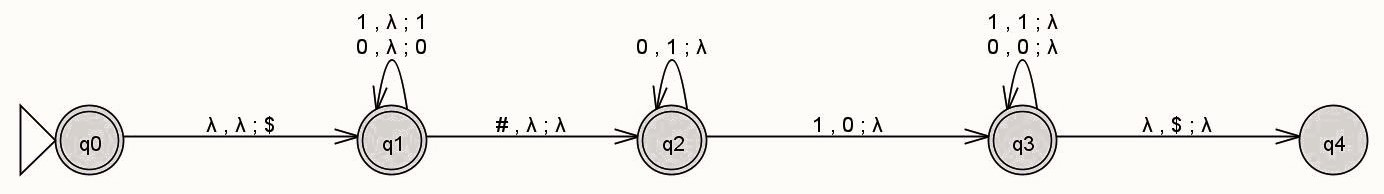
\includegraphics[width=0.9\linewidth]{Tarea 4 PDA DC.jpg}
    \label{fig:enter-label}
\end{figure}

We just present a PDA that accepts $D$ complement. It's idea basically is to check the opposite of $D$, i.e. where the string $x$ is failing. As in $D$ we have only transitions to follow the correct string, it is enough changing the accepting states. Indeed, when we don't have were to go, tracking dies and we accept in that case.

\textit{\textbf{\begin{enumerate}
    \item[3.] $E$ is not a CFL.
\end{enumerate}}}

\textbf{Proof:} We can establish this by applying the pumping lemma to an appropriate string $w \in L$. For example, $[i]_2 = 1^p 0^p$. Then the successor will be $[i +1 ]_2 = 1^p 0^{p-1}1$. So, if $E$ was a CFL then there would be $s  = 1^p 0^p \# 1^p 0^{p-1}1$ and by the CFL pumping lemma we could divide $ s = uvxyz$. By the pumping lemma we can chose $|vxy| \geq p$ where $|vy| \geq 1$. Then it is easy to see that no matter how we choose vxy such that if we change $i$ we need to change $i+1$ and the only way to do that and keep the form $string\#string$ is for $x = \#$. But even this way if we pump the last bits of $i$ and the first bits of $i+1$ we would still not satisfy $uv = i$ and $y^lz = i+1$. Because we are adding different significant bits to each number.

\textbf{\textit{\begin{enumerate}
    \item[4.] $\overline{E}$ is a CFL.
\end{enumerate}}}

We can interpret $i$ as having a sequence of 1s at its end, and $i+1$ as having a 1 followed by a sequence of 0s of the same length as the 1-run in $[i]_2$. To summarize the transformation from $[i]_2$ to $[i+1]_2$: $[i]_2$ takes the form $1w01^k$ where $k \geq 0$ is a block of 1s, and subsequently, $[i + 1]_2 = 1w10^k$ (meaning the 1s until the first 0 are changed to 1, and the 0 is changed to 1). The exceptions occur when $[i]_2 = 1^k$ for $k \geq 1$, resulting in $[i + 1]_2 = 10^k$, or when $[i]_2 = 0$, leading to $[i + 1]_2 = 1$.

Now, we examine various scenarios where a string $w$ does not belong to the language $E$, and these situations can be expressed through a context-free grammar (CFG):

\begin{enumerate}
  \item The string $w$ contains either zero or more than one occurrence of the symbol $\#$. 

For the following cases, we assume $w = x\# y$.

  \item Either $x$ or $y$ is the empty string ($\varepsilon$).
  \item $x$ is 0, but $y$ is not equal to 1.
  \item Either $x$ or $y$ begins with 0.
  \item $x = 1w01^k$, but $y$ does not equal $1w10^k$.

  To elaborate on the last case, it is noteworthy that we do not need to exclude other negative instances already addressed. Thus, the final case can be encompassed by subcases:
  \begin{itemize}
    \item $x = w01^k$ and $y = w'$, where $w$, $w'$ are arbitrary, and $z$ has a length of $k$ and includes at least one occurrence of 1.
    \item $x = w01^k$ and $y = w'0z$, where $w$, $w'$, and $z$ have lengths of $k$ and are otherwise arbitrary.
    \item $x = wz$ and $y = w'z'$, where $|z| = |z'|$, $z$ contains a 0, and $w$ is not identical to $w'$.
  \end{itemize}

  To handle the last sub-case, it is beneficial to refer to the solution for strings that do not follow the pattern $xx$ in the exercises solved in EARs homework solutions.
  \(\ \ \ \ \ \ \blacksquare\)
\end{enumerate}


\end{document}

